\begin{frame}{Система эквивалентных спинов}
  \begin{figure}
    \begin{subfigure}[t]{0.32\textwidth}
      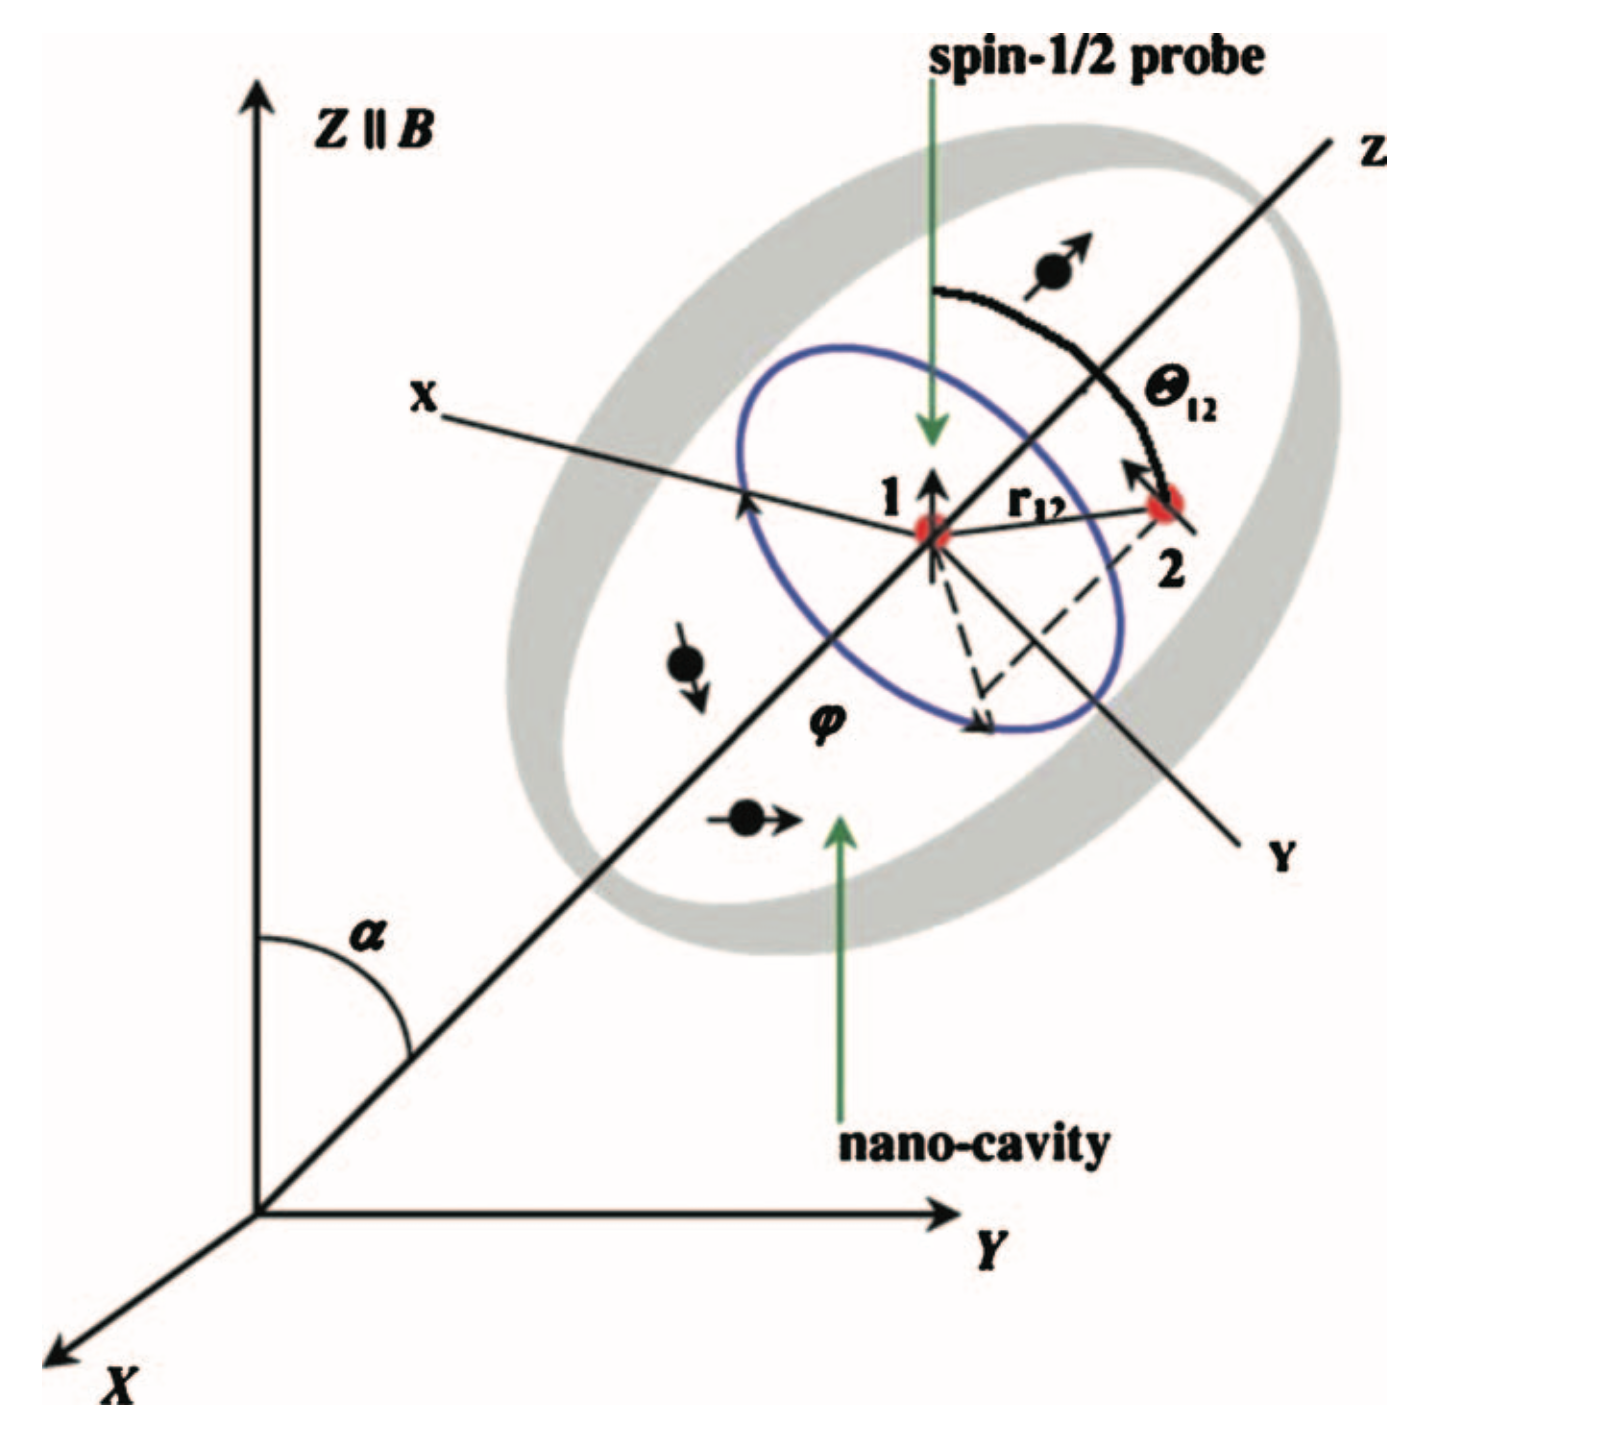
\includegraphics[width=\textwidth]{model-nanopore-schema.png}
      \caption{
        Hанопора\footnote[frame]{J. Baugh, A. Kleinhammes, D. Han, Q. Wang, and Y. Wu, \textit{Science} \textbf{294}, 1505 (2001).}
        со спин-несущих молекулами во внешнем сильном магнитном поле $\vec B$.
      }
    \end{subfigure}
    \hfill
    \begin{subfigure}[t]{0.32\textwidth}
      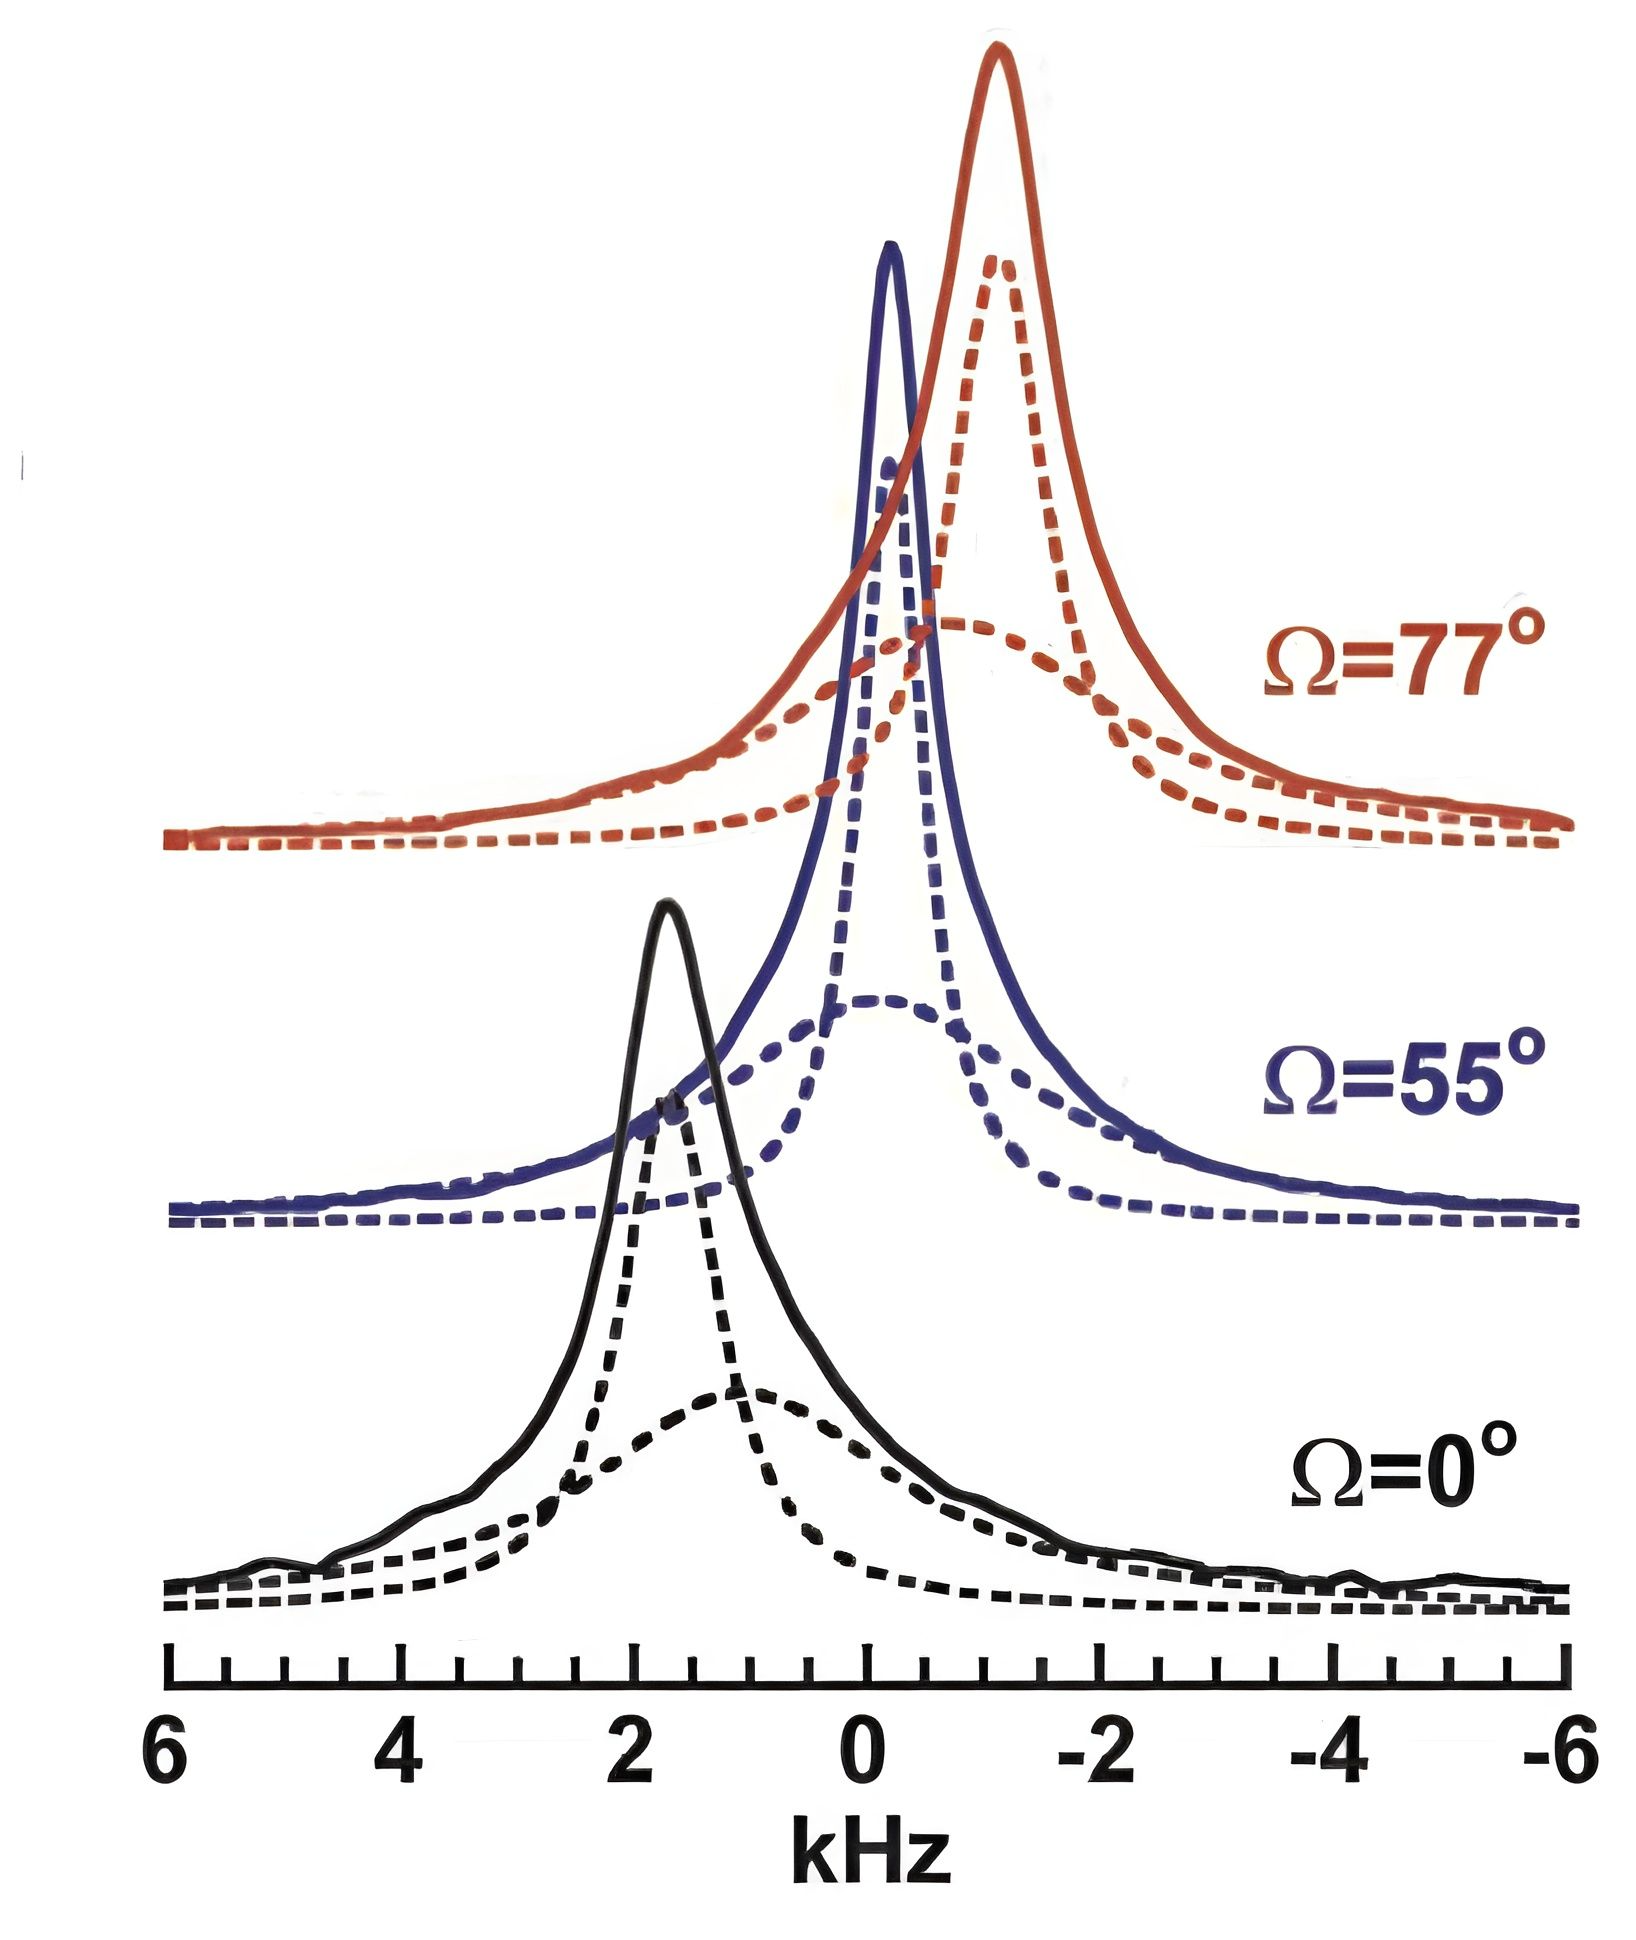
\includegraphics[width=0.8\textwidth]{sample-nanopore-nmr-spectrum.png}
      \caption{
        Молекулярная диффузия газа быстрее флип-флоп процессов.
        Вся система характеризуется одной константой $D$.
      }
    \end{subfigure}
    \hfill
    \begin{subfigure}[t]{0.32\textwidth}
      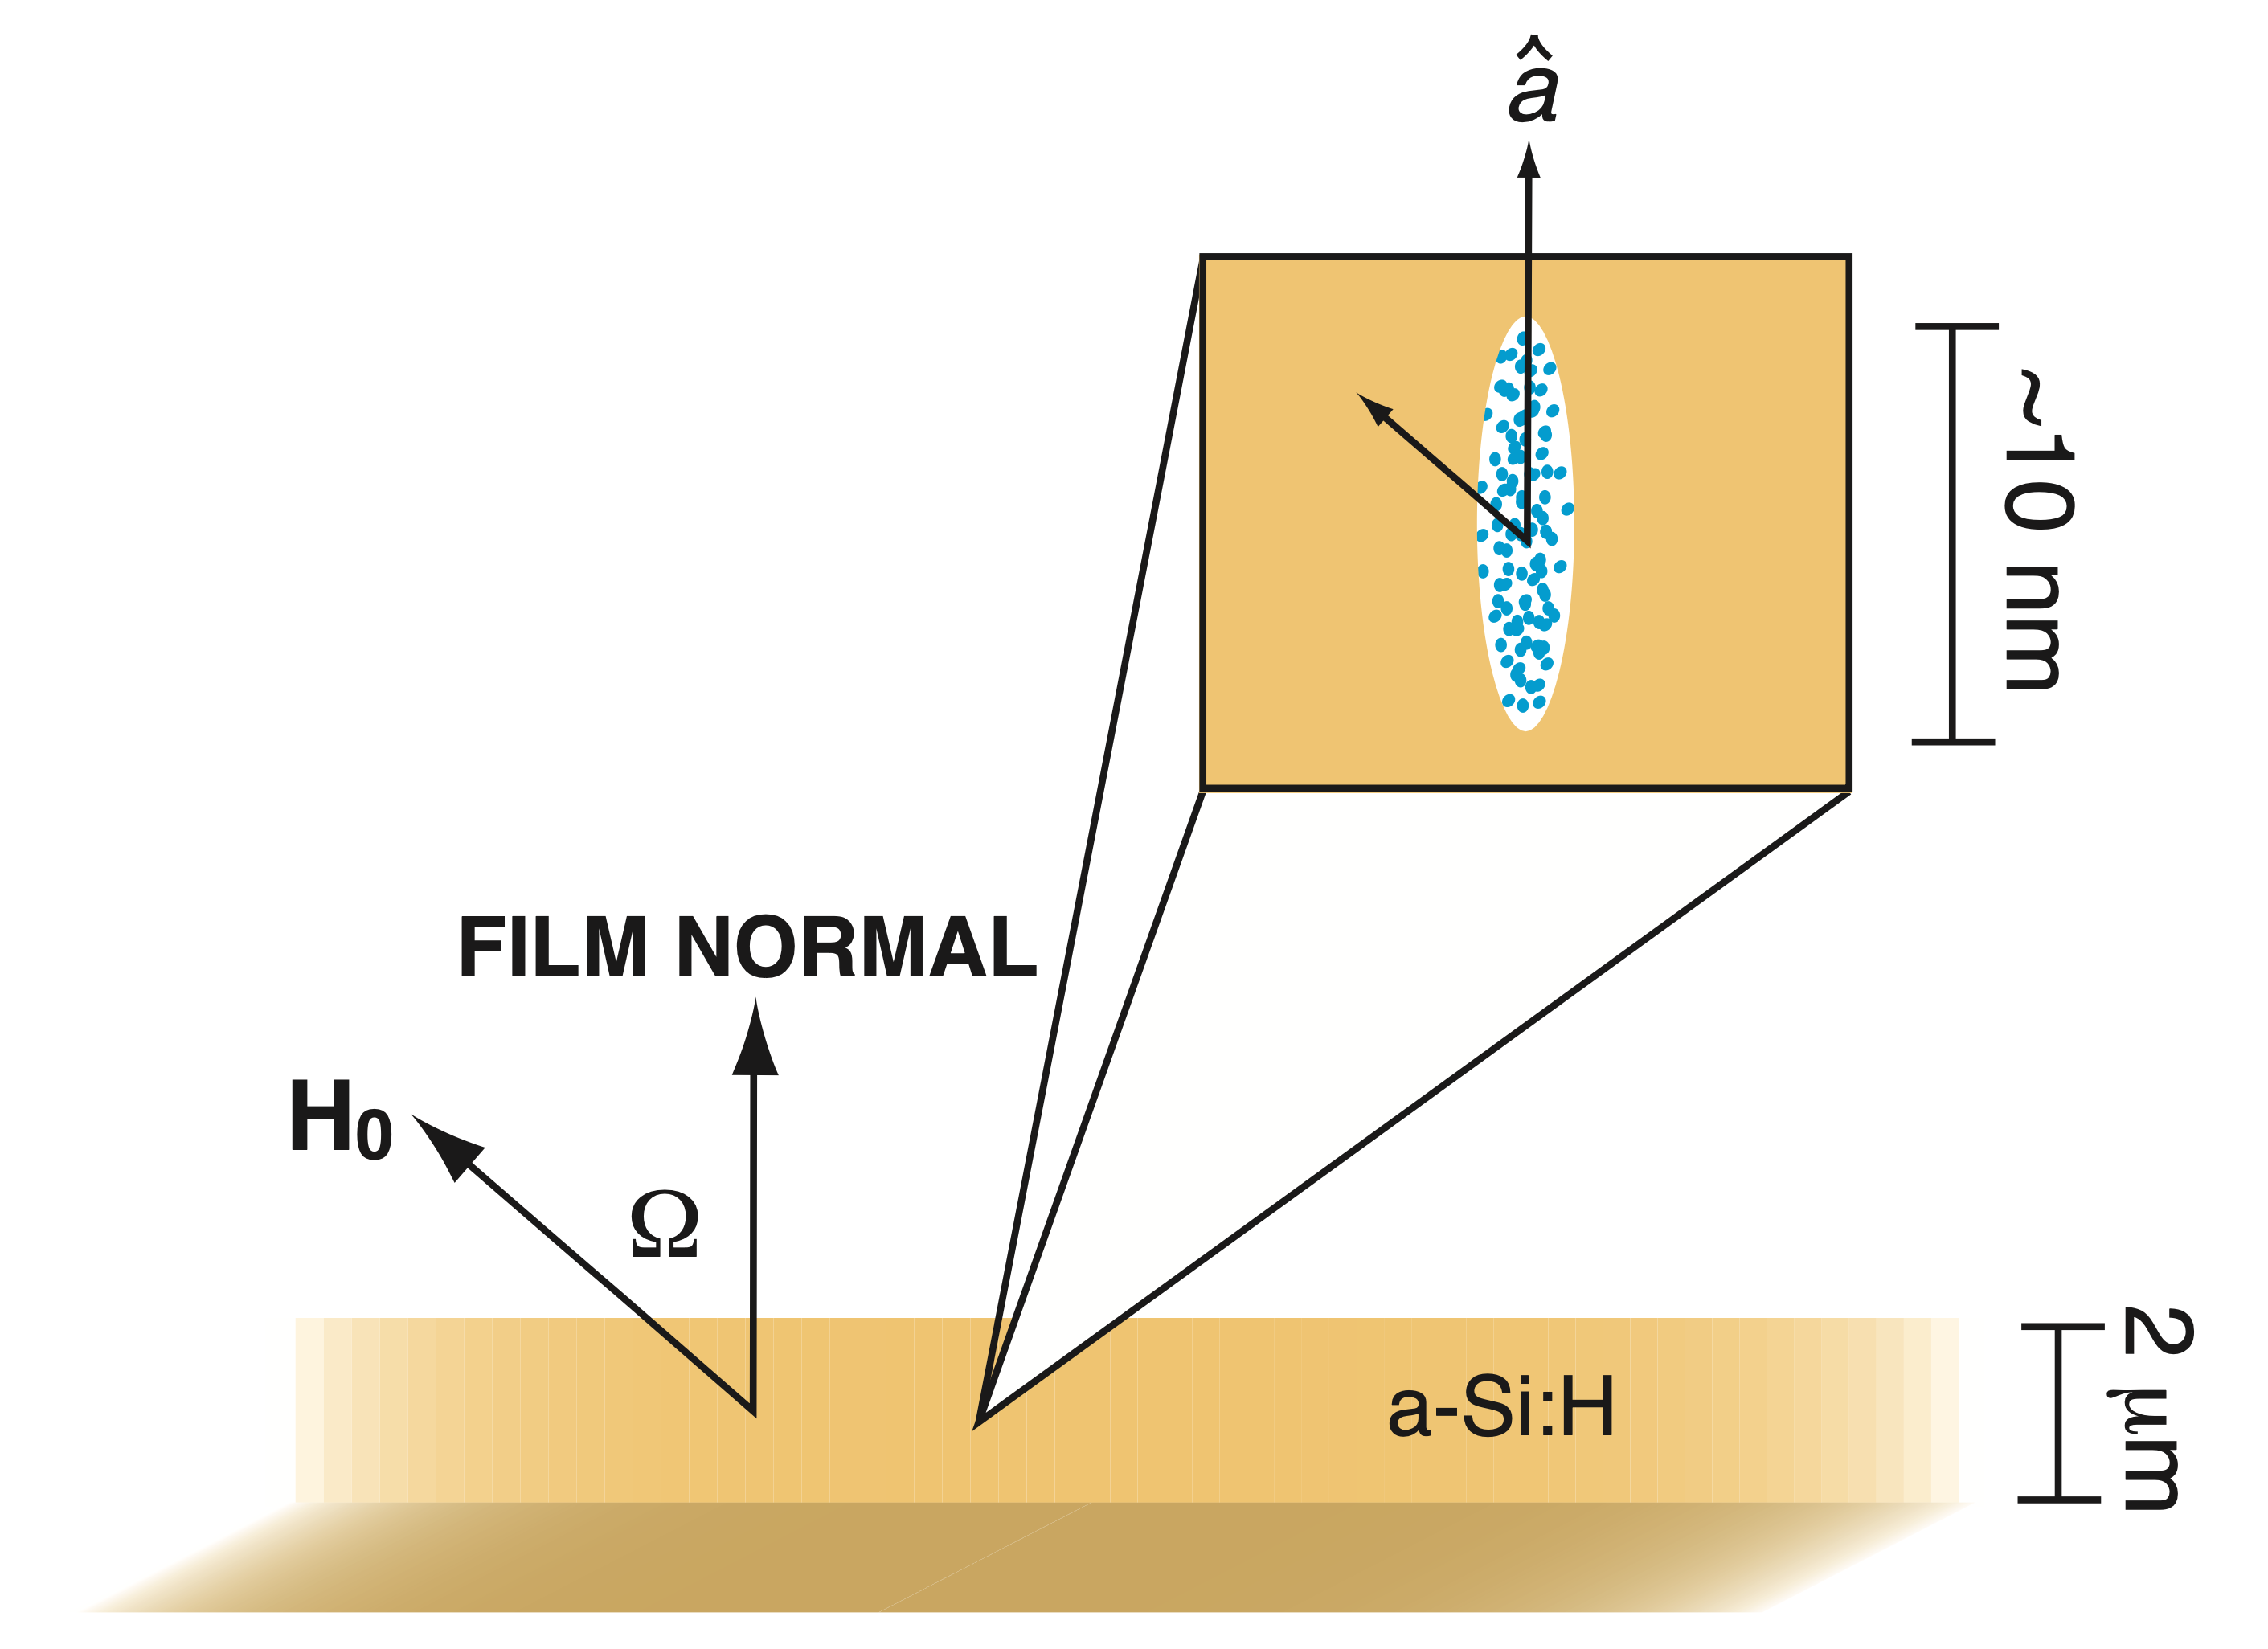
\includegraphics[width=\textwidth]{sample-nanopore-film.png}
      \caption{
        Значение константы связи $D$ зависит как от газа,
        так и от эффективного давления в нанопоре ($\approx 1$ кБар)
      }
    \end{subfigure}
    \captionsetup{skip=-0.1mm}
    \caption{}
  \end{figure}

  % \begin{block}{Нанопора\footnote[frame]{J. Baugh, A. Kleinhammes, D. Han, Q. Wang, and Y. Wu, Science 294, 1505 (2001).}, заполненая частицами со спином $1/2$}
  %     Так как молекулярная диффузия газа быстрее флип-флоп процессов,
  %     вся система характеризуется одной константой взаимодейсвия $D$.
%
  %     \vspace{\baselineskip}
%
  %     Значение константы связи $D$ зависит как от газа, так и от эффективного давления в нанопоре ($\approx 1$ кБар).
  % \end{block}
\end{frame}
\note{
    Hydrogenated amorphous silicon (Гидрогенизированный аморфный кремний)

    Для исследования многочастичной запутанности нам нужна модель,
    в которой почти все частицы взаимодействуют друг с другом,
    а также она должна поддаваться счету.
    Мы решили рассмотреть модель эквивалентных спинов.
    Такой модели соотвествует нанопора заполеннея спин несущими частицами.

    Такие нанопоры получаются выдавлием под давлением ~ 1 кБар  на специальной подложке.

    Необходимо подчеркнуть, что существуют некоторые ограничения для реализации описанной модели при исследовании нанопористых соединений с МК - ЯМР-методами. Например, модель предполагает, что все нанопоры имеют одинаковый объем и одинаковую "несферическую" форму.

    Молекулярная диффузия газа очень быстрая в сравнениидиподьных флип флом процессов
    Каждая частица успевает обойти всю нанопору пока пройдет флипфлоп
    Поэтому можно описать взаимодействие с одной константой

    Среднняя константа связи зависит как от газа, так и от эффективного давления в нанопоре

    При низких температурах диффузия побеждает?
    Какие частицы?
}
